\section{Disoccupazione}
Nella prima parte del dossier vengono riportate le analisi sulla disoccupazione e sul mercato del lavoro estrapolate da un rapporto di sintesi dell’attività analitica del Gruppo di lavoro interdipartimentale per il Monitoraggio della disoccupazione in Ticino intitolato “Ai margini del mercato del lavoro”. I dati del rapporto fanno riferimento al 2014 e vengono rappresentati in modo chiaro e sintetico permettendo una facile lettura della situazione ticinese e della situazione nazionale. Nella seconda parte del dossier si tratterà come caso pratico La Posta; verranno fornite delle informazioni generali e saranno riportati degli articoli sulle nuove tecnologie integrate dalla Posta in Svizzera e Ticino, attraverso dei dati richiesti alla posta si spera sia possibile collegare concretamente la prima parte del dossier con la seconda portando così il discorso verso le conclusioni che conteranno delle riflessioni personali, delle constatazioni che il lavoro svolto ha fatto emergere e si risponderà alla domanda di ricerca.
\subsection{Carenza di lavoro}
Secondo il documento intitolato “Ai margini del mercato del lavoro”, per fini analitici è preferibile estendere la definizione di disoccupato verso quella di carenza di lavoro. In questo modo è possibile indentificare tre categorie di forza lavoro ticinese toccate dalla disoccupazione. Nella prima categoria si trovano i disoccupati, iscritti o non agli Uffici Regionali di Collocamento (URC), ovvero quelle persone senza impiego e alla ricerca attiva di un lavoro; in Ticino nel 2014 si stimarono 11'983 persone disoccupate. Nella seconda si trovano invece i sottoccupati, ossia persone occupate a tempo parziale che vorrebbero incrementare il proprio grado d’impiego; in Ticino sempre nel 2014 si stimarono 14'676 sottoccupati. Infine nella terza categoria si trovano gli scoraggiati, persone senza impiego, che sarebbero disposte a lavorare, ma che dichiarano di non aver cercato lavoro perché convinti di non riuscire a trovarlo; in Ticino nel 2014 si stimarono 235 casi.
\subsection{Evoluzione della disoccupazione}
\subsubsection{Definizioni}
In Svizzera esistono due differenti definizioni di disoccupati:
disoccupati iscritti agli URC: persone senza un impiego e immediatamente collocabili, registrate presso un Ufficio Regionale di Collocamento indipendentemente dal fatto che percepiscano o meno un’indennità di disoccupazione;
disoccupati ai sensi dell’ILO (International Labour Organization): persone in età compresa tra i 15 e i 74 anni che rispondono contemporaneamente alle seguenti condizioni:
non erano occupate nel corso della settimana di riferimento;
hanno cercato attivamente impiego nelle quattro settimane precedenti;
erano disposte a iniziare subito un’attività.
\subsubsection{Provenienza dati}
Di riflesso esistono due diverse fonti di riferimento:
archivi della Seco, basata sui disoccupati iscritti agli Uffici Regionali di Collocamento;
quelle definite secondo i criteri dell’Organizzazione Interazionale del Lavoro (ILO), i cui numeri sono stimati dalla Rivelazione sulle Forze di lavoro in Svizzera (RIFOS) dell’Ufficio federale di statistica (UST).
\subsubsection{Analisi svolta}
Queste fonti e i loro dati vengono analizzati e rielaborati nel documento intitolato “Ai margini del mercato del lavoro”, rapporto di sintesi dell’attività analitica del Gruppo di lavoro interdipartimentale per il Monitoraggio della disoccupazione in Ticino.
In Ticino nel 2014 si stimarono quasi 12'000 disoccupati di cui solo circa la metà erano iscritti presso un URC. Grazie ai dati della Seco, si è constatato che in Ticino tra il 2002 e il 2014 il numero di disoccupati iscritti agli URC è aumentato non in maniera lineare da 5'136 a 6'810 casi e il rispettivo tasso di disoccupazione dal 3.5% al 4.2%.
\begin{figure}
    \centering
    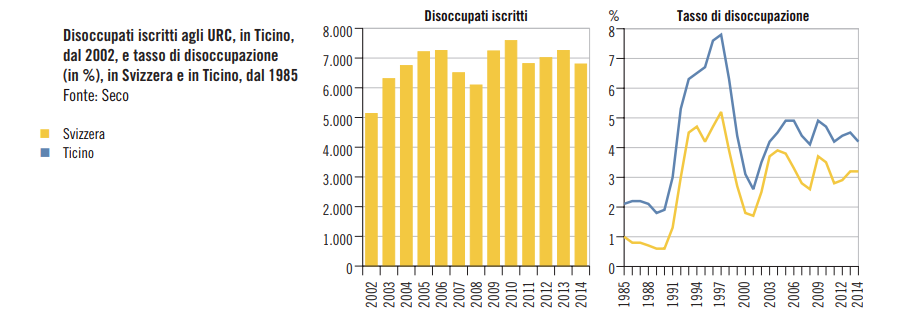
\includegraphics{Disoccupati iscritti agli URC.png}
    \caption{Caption}
    \label{Disoccupati iscritti agli URC, in Ticino, dal 2002 e tasso di disoccupazione}
\end{figure}
La dinamica ticinese è stata messa a confronto con quella nazionale e sono emerse alcune conferme:
il tasso di disoccupazione in Ticino è tendenzialmente più alto rispetto a quello nazionale,
i tassi di disoccupazione misurati a livello svizzero e cantonale sembrano muoversi nella stessa direzione e ciò indica come la dinamica ticinese sia interconnessa a quella nazionale;
il tasso di disoccupazione ticinese presenta oscillazioni stagionali più marcate rispetto all’andamento nazionale. Questa differenza è data dalla struttura dell’economia ticinese che è caratterizzata da settori a carattere stagionale come il turismo o le costruzioni che influenzano in modo marcato e regolare l’andamento del numero di disoccupati.
In Ticino nel 2014 si stimò che i disoccupati ai sensi dell’ILO erano poco meno di 12'000 e il tasso era del 6.7%. Anche in questo caso la disoccupazione è aumentata anche se non in modo lineare rispetto ai valori del 2002.
\begin{figure}
    \centering
    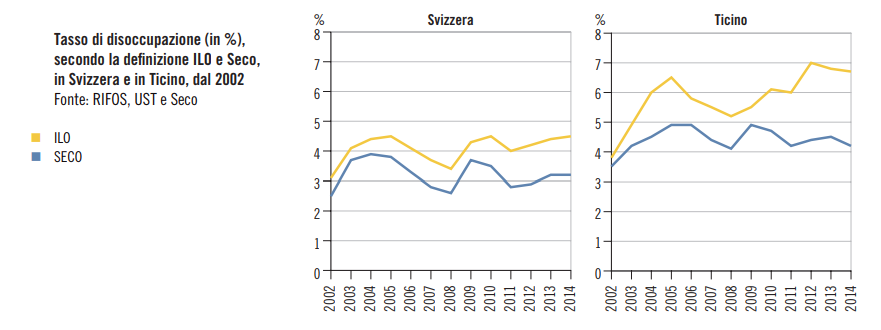
\includegraphics{Tasso di disoccupazione secondo ILO e Seco.png}
    \caption{Caption}
    \label{Tasso di disoccuapzione secondo ILO e Seco}
\end{figure}
\textbf{In sintesi} le tradizionali statistiche danno un quadro parziale della realtà del fenomeno della disoccupazione. In Ticino circa la metà delle persone disoccupate che si dichiara tale è iscritta agli URC. Negli ultimi anni in Ticino il tasso di disoccupazione secondo i criteri ILO è cresciuto più rapidamente rispetto al tasso nazionale e il divario tra il tasso ILO ticinese e quello svizzero è progressivamente aumentato.